\documentclass[12pt,UTF8]{ctexart}
\usepackage{ctex,amsmath,amssymb,geometry,fancyhdr,bm,amsfonts,mathtools,extarrows,graphicx,url,enumerate,xcolor,float,multicol,wasysym}
\usepackage{subfigure}
\allowdisplaybreaks[4]
% 加入中文支持
\newcommand\Set[2]{\left\{#1\ \middle\vert\ #2 \right\}}
\newcommand\Lim[0]{\lim\limits_{n\rightarrow\infty}}
\newcommand\LIM[2]{\lim\limits_{#1\rightarrow#2}}
\newcommand\Ser[1]{\sum_{n=#1}^\infty}
\newcommand{\SER}[2]{\sum_{#1=#2}^\infty}
\newcommand{\Int}[4]{\varint\nolimits_{#1}^{#2}#3\mathrm d#4}
\newcommand{\aIInt}[1]{\iint\limits_{#1}}
\newcommand{\IInt}[3]{\iint\limits_{#1}#2\mathrm d#3}
\newcommand{\varIInt}[4]{\iint\limits_{#1}#2\mathrm d#3\mathrm d#4}
\newcommand{\IIInt}[3]{\iiint\limits_{#1}#2\mathrm d#3}
\newcommand{\varIIInt}[5]{\iiint\limits_{#1}#2\mathrm d#3\mathrm d#4\mathrm d#5}
\newcommand{\LInt}[3]{\varint\nolimits_{#1}#2\mathrm d#3}
\newcommand{\LOInt}[3]{\varoint\nolimits_{#1}#2\mathrm d#3}
\newcommand{\LLInt}[4]{\varint\nolimits_{#1}\nolimits^{#2}#3\mathrm d#4}
\newcommand{\BLInt}[2]{\varint\nolimits_{#1}#2}
\newcommand{\varBLInt}[3]{\varint\nolimits_{#1}\nolimits^{#2}#3}
\newcommand{\BLOInt}[2]{\varoint\nolimits_{#1}#2}
\newcommand{\SIInt}[3]{\iint\limits_{#1}#2\mathrm d#3}
\newcommand{\md}[1]{\mathrm d#1}
\newcommand{\BSIInt}[2]{\iint\limits_{#1}#2}
\newcommand{\pp}[2]{\frac{\partial #1}{\partial #2}}
\newcommand{\ppx}[1]{\frac{\partial #1}{\partial x}}
\newcommand{\ppy}[1]{\frac{\partial #1}{\partial y}}
\newcommand{\ppz}[1]{\frac{\partial #1}{\partial z}}
\newcommand{\varppx}[1]{\frac{\partial}{\partial x} #1}
\newcommand{\varppy}[1]{\frac{\partial}{\partial y} #1}
\newcommand{\varppz}[1]{\frac{\partial}{\partial z} #1}
\newcommand{\BSOIInt}[2]{\oiint\limits_{#1}#2}
\newcommand{\me}[0]{\mathrm e}
\geometry{a4paper,scale=0.80}
\pagestyle{fancy}
\rhead{向量场的微积分(1)}
\lhead{基础习题课期末复习}
\chead{微积分B(2)}
\begin{document}
\setcounter{section}{9}
\section{第二型曲线积分、格林公式}
\noindent
\subsection{复习计划}
\begin{figure}[H]
\begin{center}
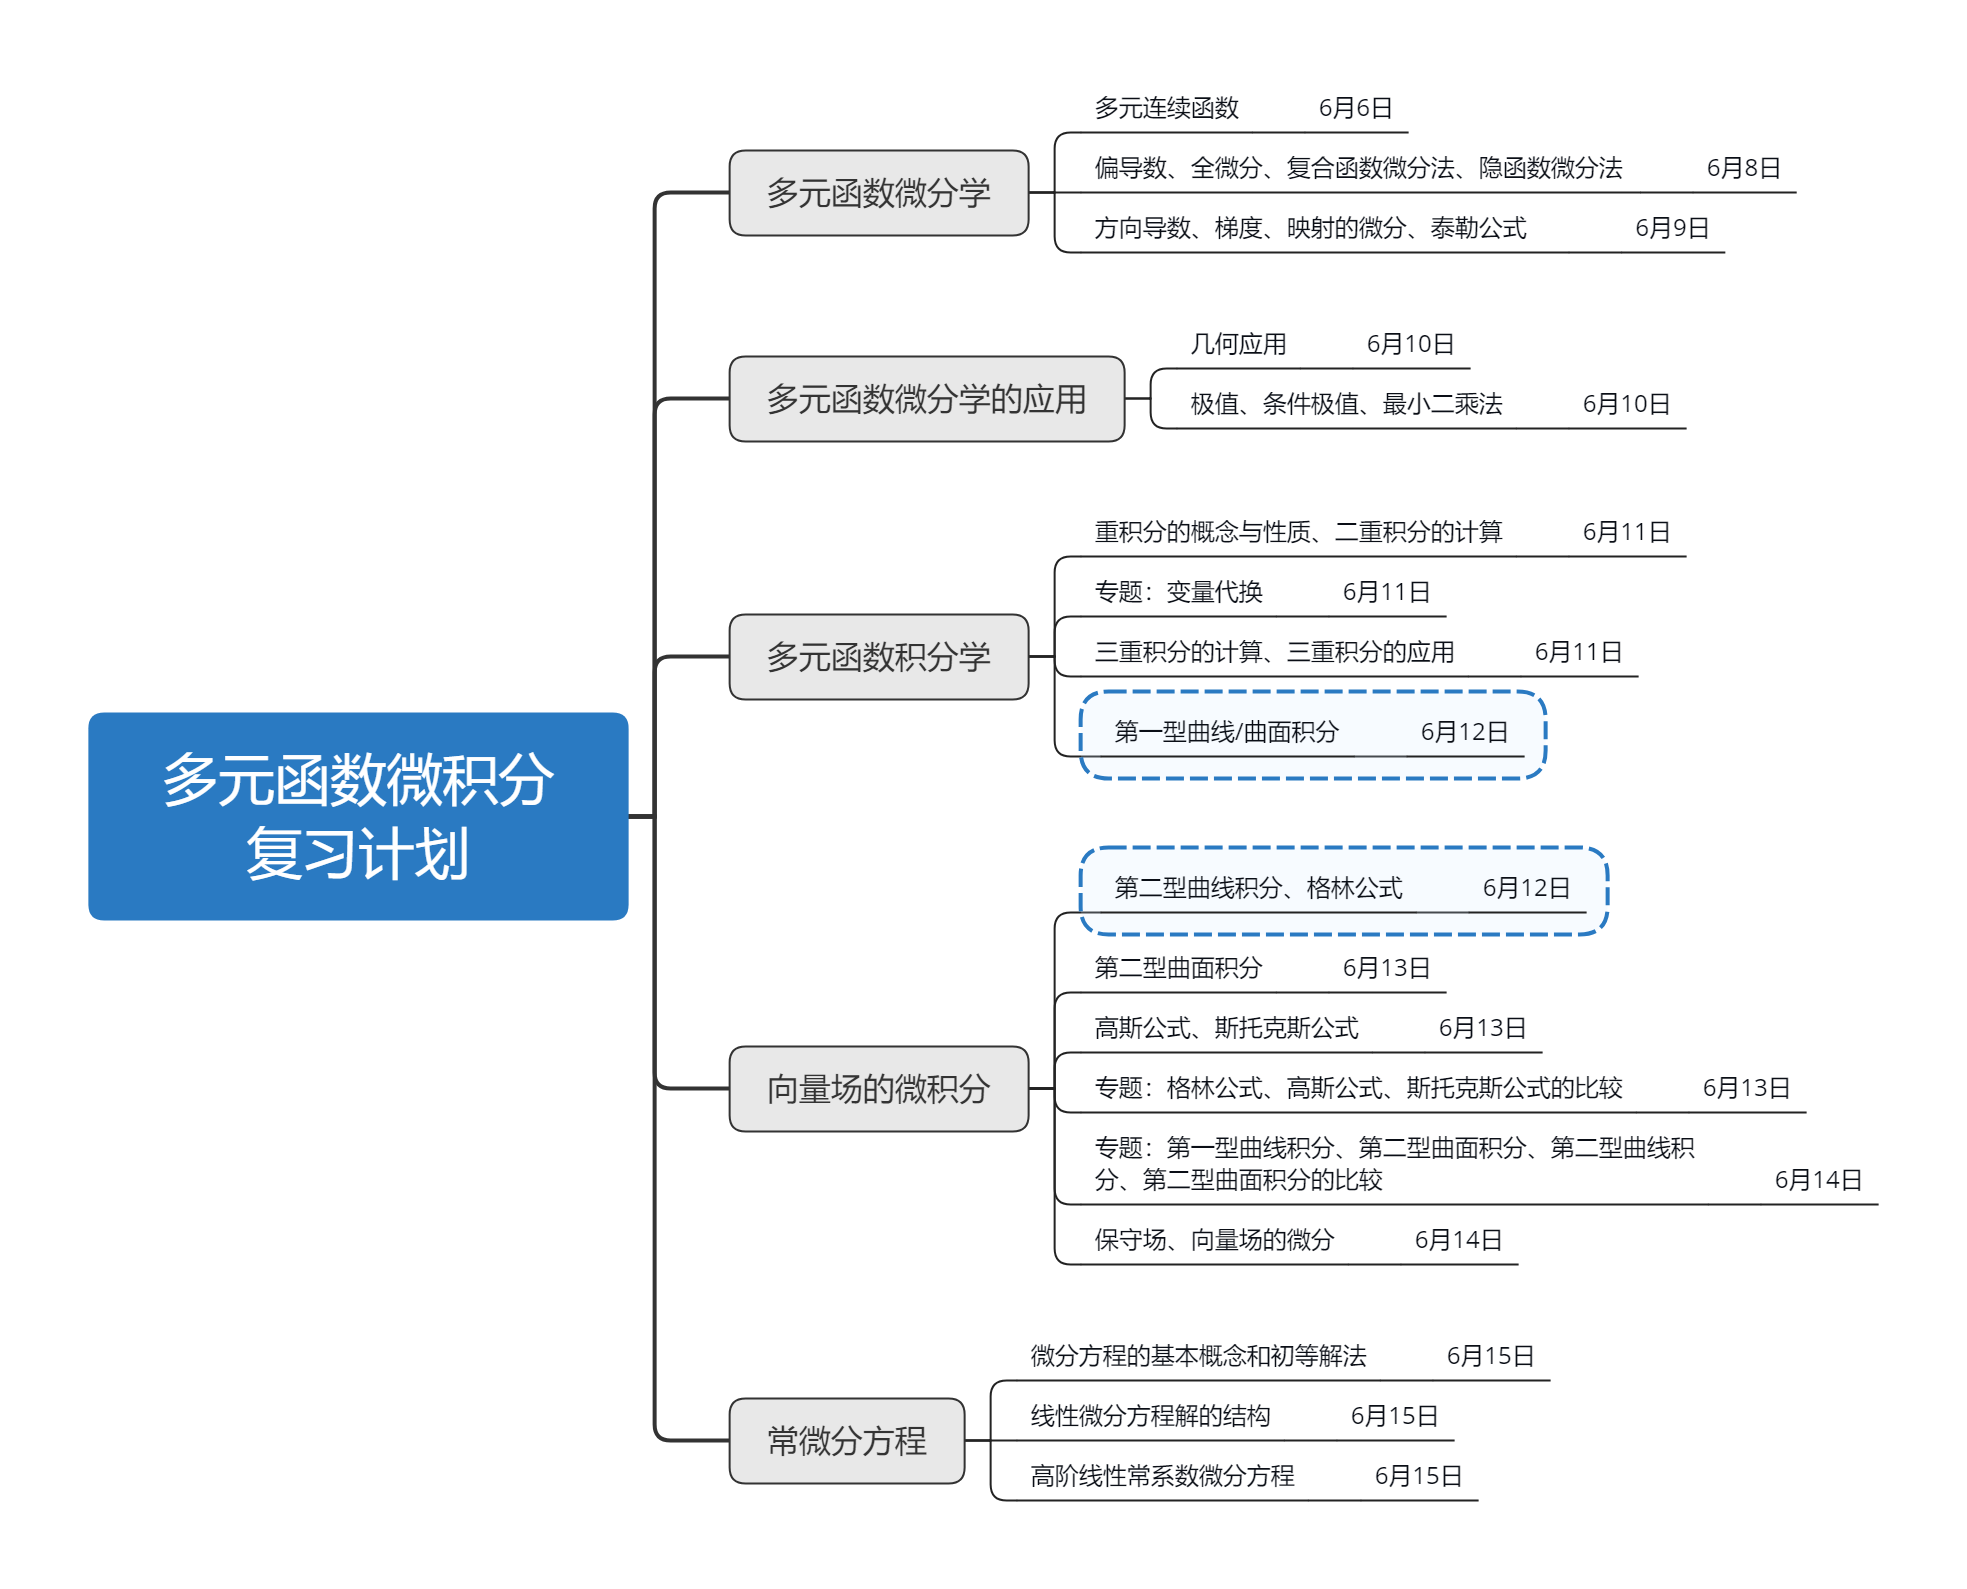
\includegraphics[height=0.5\textheight]{Figures20190612/plan.png}
\end{center}
\end{figure}
\subsection{知识结构}
\begin{figure}[H]
\begin{center}
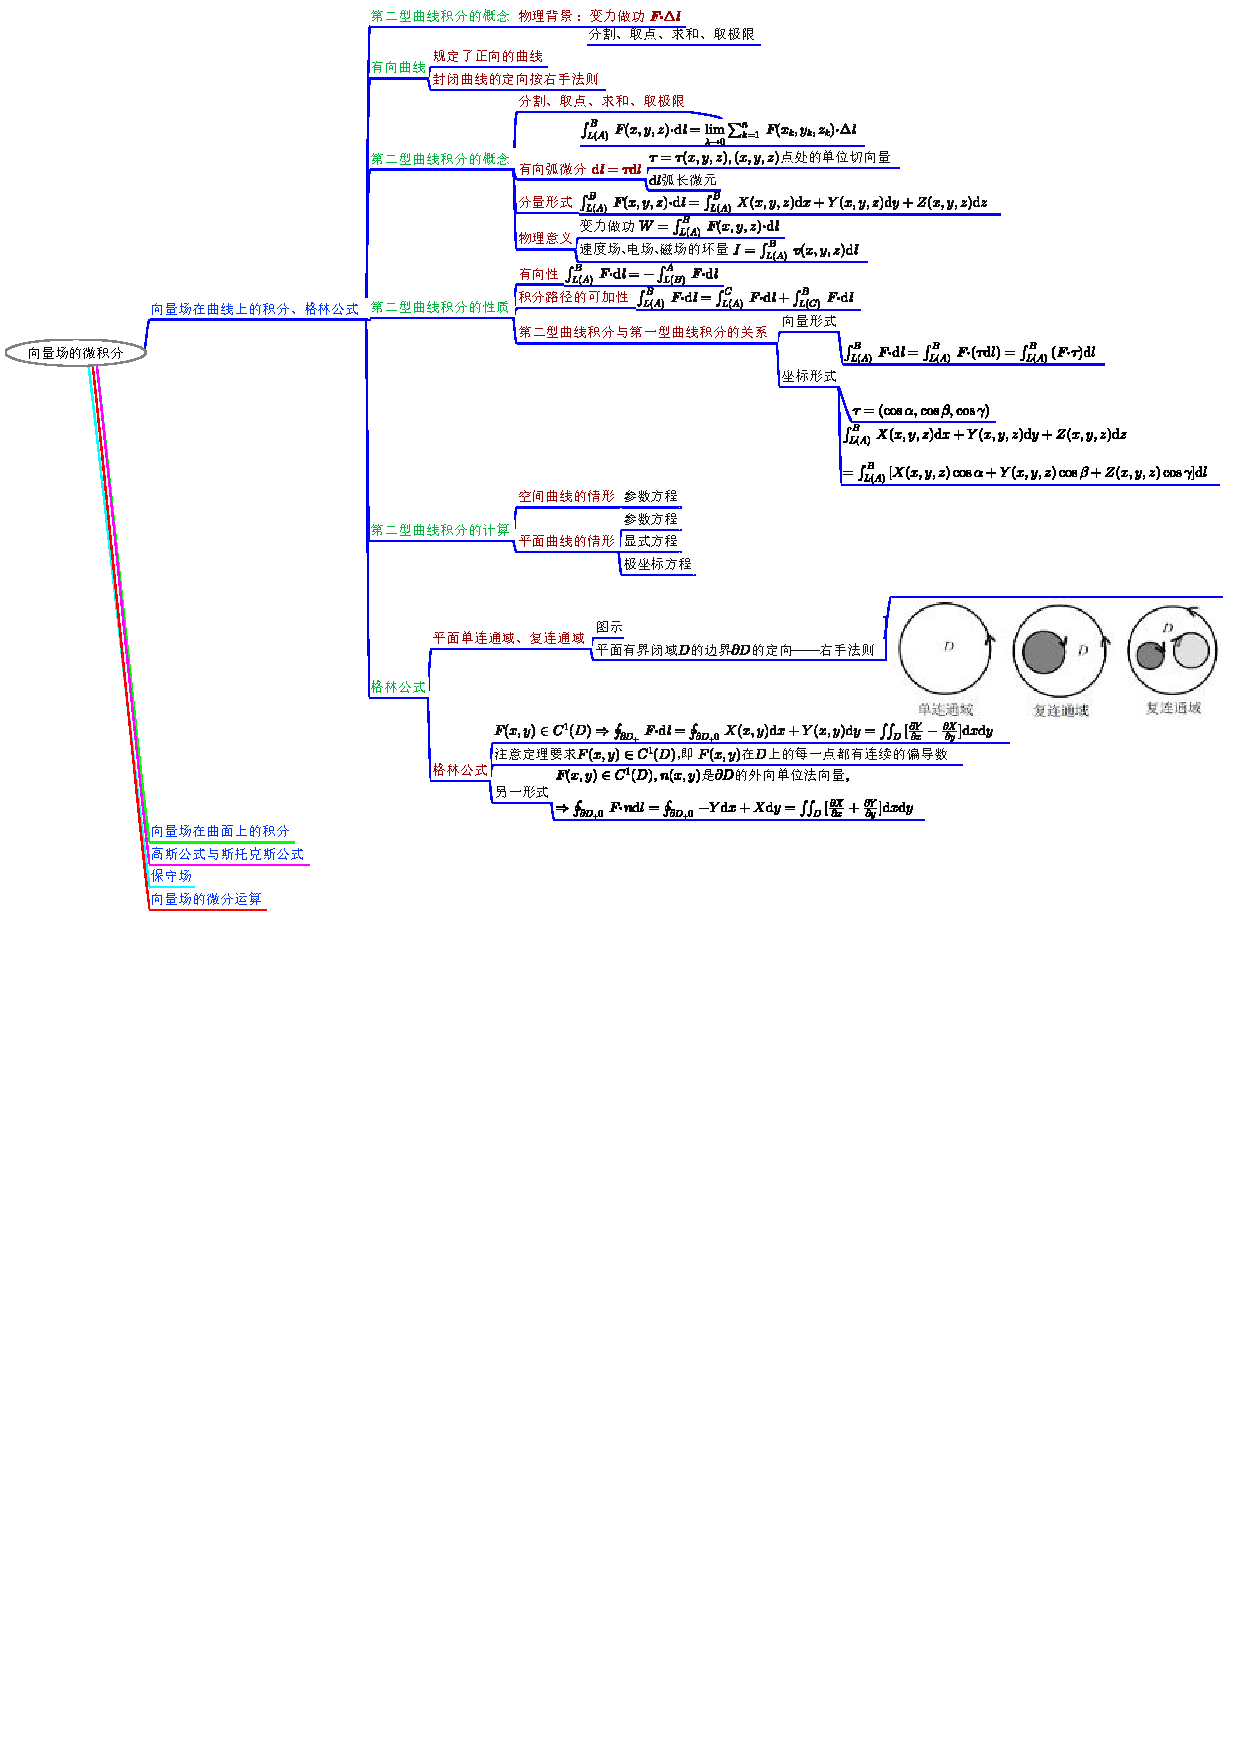
\includegraphics[height=1\textheight,angle=0]{20190612-1.pdf}
\end{center}
\end{figure}
\subsection{重要知识}
第二型曲线积分是为了计算力在曲线路径上做功的问题引入的,是向量场在曲线路径上的积分. 第一型曲线积分是数量场在曲线路径上的积分,要注意第二型曲线积分与第一型曲线积分的区别.
\begin{enumerate}
\item第二型曲线积分的计算
\begin{enumerate}
\item空间曲线——已知参数方程:\\
\[\begin{aligned}
&L:\begin{cases}x=x(t),\\ y=y(t),\\ z=z(t),\end{cases}t\in[\alpha,\beta], A: t=\alpha, B: t=\beta, \bm F(x,y,z)\in C(L),\\
\Rightarrow&\varint_{L(A)}^B\bm F(x,y,z)\bm\cdot\mathrm d\bm l=\varint_{L(A)}^BX(x,y,z)\mathrm dx+Y(x,y,z)\mathrm dy+Z(x,y,z)\mathrm dz\\
&=\varint_\alpha^\beta[X(x(t),y(t),z(t))x'(t)+Y(x(t),y(t),z(t))y'(t)+Z(x(t),y(t),z(t))z'(t)]\mathrm dt
\end{aligned}\]
\item平面曲线
\begin{enumerate}
\item已知参数方程:\\
\[\begin{aligned}
&L: \begin{cases}x=x(t),\\ y=y(t)\end{cases}, t\in[\alpha,\beta], A: t=\alpha, B: t=\beta, \bm F(x,y)\in C(L),\\
\Rightarrow&\varint_{L(A)}^B\bm F(x,y)\bm\cdot\mathrm d\bm l=\varint_{L(A)}^BX(x,y)\mathrm dx+Y(x,y)\mathrm dy\\
&=\varint_\alpha^\beta[X(x(t),y(t))x'(t)+Y(x(t),y(t))y'(t)]\mathrm dt
\end{aligned}\]
\item已知显式方程:
\[\begin{aligned}
&L: y=f(x)\in C[a,b], A: x=a, B: x=b, \bm F(x,y)\in C(L),\\
\Rightarrow&\int_{L(A)}^B\bm F(x,y)\bm\cdot\mathrm d\bm l=\int_{L(A)}^BX(x,y)\mathrm dx+Y(x,y)\mathrm dy\\
&=\int_a^b[X(x,f(x))+Y(x,f(x))f'(x)]\mathrm dx
\end{aligned}\]
\item已知极坐标方程:
\[\begin{aligned}
&L: r=r(\theta), A: t=\alpha, B: t=\beta, \bm F(x,y)\in C(L),\\
\Rightarrow&\int_{L(a)}^B\bm F(x,y)\bm\cdot\mathrm d\bm l=\int_{L(A)}^BX(x,y)\mathrm dx+Y(x,y)\mathrm dy\\
&=\int_\alpha^\beta[X(r(\theta)\cos\theta,r(\theta)\sin\theta)(r(\theta)\cos\theta)'+Y(r(\theta)\cos\theta,r(\theta)\sin\theta)(r(\theta)\sin\theta)']\mathrm d\theta
\end{aligned}\]
\end{enumerate}
\end{enumerate}
\item格林公式.
\begin{enumerate}
\item格林公式的第一个形式:
\[\textcolor{red}{\bm F(x,y)\in C^1(D)}\Rightarrow\varoint_{\partial D_+}\bm F\bm\cdot\mathrm d\bm l=\varoint_{\partial D_+}X(x,y)\mathrm dx+Y(x,y)\mathrm dy=\iint_D[\frac{\partial Y}{\partial x}-\frac{\partial X}{\partial y}]\mathrm dx\mathrm dy\]
\item格林公式的第二个形式:
\[\begin{aligned}
&\textcolor{red}{\bm F(x,y)\in C^1(D)},\bm n(x,y)\text{是$\partial D$的外向单位法向量},\\
\Rightarrow&\varoint_{\partial D_+}\bm F\bm\cdot\bm n\mathrm dl=\varoint_{\partial D_+}-Y\mathrm dx+X\mathrm dy=\iint_D[\frac{\partial X}{\partial x}+\frac{\partial Y}{\partial y}]\mathrm dx\mathrm dy
\end{aligned}\]
\end{enumerate}
\end{enumerate}
\subsection{习题分类与解题思路}
对于第二型空间曲线积分,目前我们只有参数方程一种类型的曲线可以计算. 

对于第二型平面曲线积分,可以根据曲线的形式(参数方程、显式方程、极坐标方程),选择合适的公式计算. 

对于平面封闭曲线上的第二型曲线积分,可利用格林公式转化成二重积分,以简化计算. 应用格林公式时,须注意平面向量场的两个分量函数应在曲线围成的区域内有一阶连续偏导数,若不满足该条件,可选取简单的曲线,将偏导数不存在的点去掉,构造可以应用格林公式的区域.
\begin{enumerate}
\item第二型曲线积分.
\begin{enumerate}
\item空间曲线. 可选择合适的参数将曲线方程写成参数方程的形式,代入公式计算.

【如习题13.2中的7., 11.】
\item平面曲线
\begin{enumerate}
\item显式方程

【如习题13.2中的2., 5.(折线路径,积分路径可加性), 6.(折线路径,积分路径可加性), 8.(折线路径,积分路径可加性)】
\item极坐标方程

【如习题13.2中的3., 4.】
\item参数方程

【如习题13.2中的1.】
\end{enumerate}
\item在计算之前要利用曲线方程将被积函数适当化简.

【如习题13.2中的3., 4., 5., 8.】
\item利用对称性可简化计算.

【如习题13.2中的9.(轮换对称性)】
\item考查第二型曲线积分的物理意义. (力在曲线路径上做功.)

【如习题13.2中的10.】
\end{enumerate}
\item格林公式.
\begin{enumerate}
\item直接代入公式$\BLOInt{\partial D}{X(x,y)\mathrm dx+Y(x,y)\mathrm dy}=\IInt D{(\ppx Y-\ppy X)}xy$计算. 函数$X(x,y),Y(x,y)$应满足一阶偏导数连续的条件. 初等函数的偏导数在定义域均满足连续的条件,需要注意初等函数定义域外的点.

【如习题13.3中的1.(1)/(2)/(3)/(4)/(5)/(6)/(7), 2.(1)., 3.(1)/(2)】
\item考查函数$X(x,y),Y(x,y)$应满足一阶偏导数连续的条件这一点. 可选取简单曲线将偏导函数的间断点去掉. 这一点会在格林公式、高斯公式、斯托克斯公式的专题中进行总结.

【如习题13.3中的2.(2)】
\item考查格林公式的第二个形式.

【如习题13.3中的4.】
\end{enumerate}
\end{enumerate}
\subsection{习题13.2解答}
\begin{enumerate}
\item计算$\BLInt L{(x+y)\mathrm dx-(x-y)\mathrm dy}$,其中$L$为椭圆$\frac{x^2}{a^2}+\frac{y^2}{b^2}=1$的上半周,逆时针方向为正.

解:$\BLInt L{(x+y)\mathrm dx-(x-y)\mathrm dy}=\varBLInt0\pi{(a\cos\theta+b\sin\theta)\mathrm d(a\cos\theta)-(a\cos\theta-b\sin\theta)\mathrm d(b\sin\theta)}\\
=\Int0\pi{(-a^2\sin\theta\cos\theta-ab\sin^2\theta-ab\cos^2\theta+b^2\sin\theta\cos\theta)}\theta\\
=(b^2-a^2)\Int0\pi{\sin\theta\cos\theta}\theta-ab\Int0\pi{}\theta=0-\pi ab=-\pi ab$.

\item计算$\BLInt L{y^2\mathrm dx-x^2\mathrm dy}$,其中$L$为抛物线$y=x^2$自$x=-1$到$x=1$的一段.

解:$\BLInt L{y^2\mathrm dx-x^2\mathrm dy}=\varBLInt{-1}1{(x^2)^2\mathrm dx-x^2\mathrm d(x^2)}=\varBLInt{-1}1{x^4\mathrm dx-2x^3\mathrm dx}=\Int{-1}1{x^4-2x^3}\mathrm dx\\
=(\frac15x^5-\frac24x^4)\big|_{-1}^1=\frac25$.

\item计算$\BLOInt L{\frac{x\mathrm dy-y\mathrm dx}{x^2+y^2}}$,其中$L$为圆周$x^2+y^2=a^2$(逆时针方向为正).

解:$\BLOInt L{\frac{x\mathrm dy-y\mathrm dx}{x^2+y^2}}=\frac1{a^2}\BLOInt L{x\mathrm dy-y\mathrm dx}=\frac1{a^2}\varBLInt0{2\pi}{a\cos\theta\mathrm d(a\sin\theta)-a\sin\theta\mathrm d(a\cos\theta)}\\
=\frac1{a^2}\varBLInt0{2\pi}{a\cos\theta(a\cos\theta)\mathrm d\theta-a\sin\theta(-a\sin\theta)\mathrm d\theta}=\frac1{a^2}\Int0{2\pi}{(a^2\cos^2\theta+a^2\sin\theta)}\theta=2\pi$.

\item计算$\BLOInt L{\frac{y\mathrm dy-x\mathrm dx}{x^2+y^2}}$,其中$L$为圆周$x^2+y^2=a^2$(逆时针方向为正).

解:$\BLOInt L{\frac{y\mathrm dy-x\mathrm dx}{x^2+y^2}}=\frac1{a^2}\BLOInt L{y\mathrm dy-x\mathrm dx}=\frac1{a^2}\varBLInt0{2\pi}{a\sin\theta\mathrm d(a\sin\theta)-a\cos\theta\mathrm d(a\cos\theta)}\\
=\frac1{a^2}\varBLInt0{2\pi}{a\sin\theta(a\cos\theta)\mathrm d\theta-a\cos\theta(-a\sin\theta)\mathrm d\theta}=\frac1{a^2}\Int0{2\pi}{(a^2\sin\theta\cos\theta+a^2\sin\theta\cos\theta)}\theta\\
=\Int0{2\pi}{\sin\theta\cos\theta}\theta=\Int0{2\pi}{\sin\theta}{\sin\theta}=\frac12\sin^2\theta\big|_0^{2\pi}=0$.

\item计算$\BLInt L{\frac{\mathrm dx+\mathrm dy}{|x|+|y|}}$,其中$L$为由$A(0,-1)$到$B(1,0)$再到$C(0,1)$的折线.

\begin{figure}[H]
\begin{center}
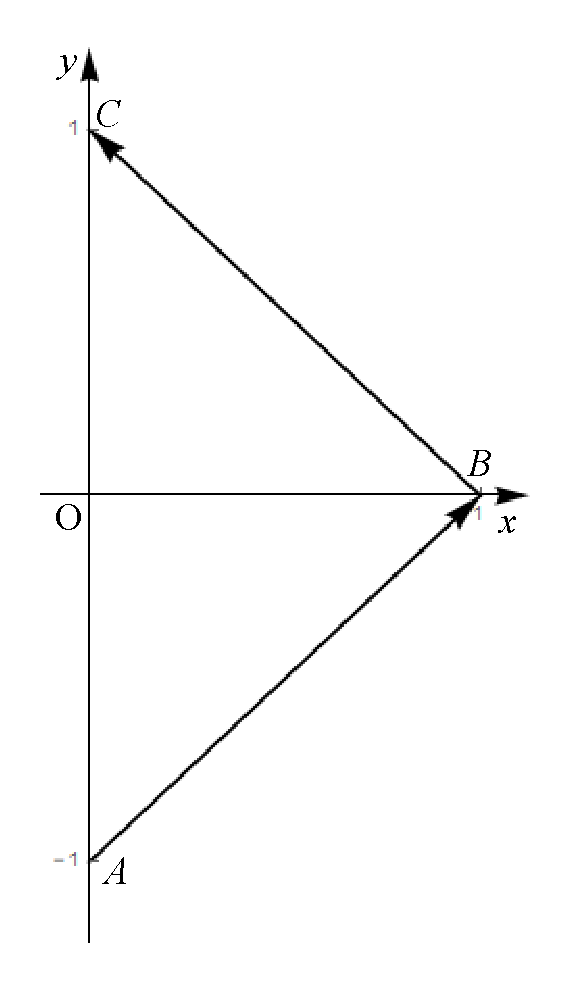
\includegraphics[height=0.3\textheight]{Figures22/Fig13-2-5.pdf}
\end{center}
\caption{习题13.2 5.题图示}
\label{13-2-5}
\end{figure}

解:$AB$段的方程为$\frac x1+\frac y{-1}=1$,即$y=x-1,x:0\rightarrow1$,$BC$段的方程为$\frac x1+\frac y1=1$,即$y=1-x,x:1\rightarrow0$,

易知折线$ABC$满足方程$|x|+|y|=1$,

$\therefore\BLInt L{\frac{\mathrm dx+\mathrm dy}{|x|+|y|}}=\BLInt L{\mathrm dx+\mathrm dy}=(\varint\nolimits_{AB}+\BLInt{BC}{)(\mathrm dx+\mathrm dy)}=\BLInt{AB}{\mathrm dx+\mathrm dy}+\BLInt{BC}{\mathrm dx+\mathrm dy}\\
=\varBLInt01{\mathrm dx+d(x-1)}+\varBLInt10{\mathrm dx+\mathrm d(1-x)}=\varBLInt01{\mathrm dx+\mathrm dx}+\varBLInt10{\mathrm dx-\mathrm dx}=2\Int01{}x+0=2$.

\item计算$\BLInt L{(x^2+y^2)\mathrm dx+(x^2-y^2)\mathrm dy}$,其中$L$为$y=1-|1-x|,x\in[0,2]$,曲线正向为$x$增长的方向.

\begin{figure}[H]
\begin{center}
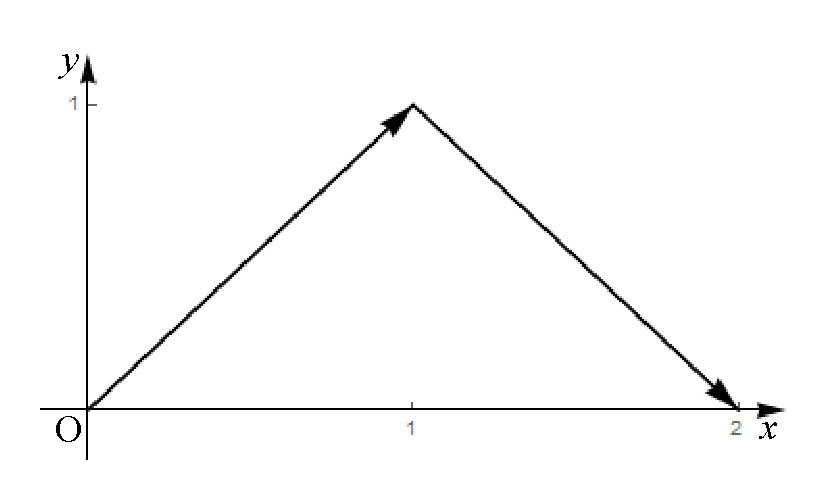
\includegraphics[height=0.2\textheight]{Figures22/Fig13-2-6.pdf}
\end{center}
\caption{习题13.2 6.题图示}
\label{13-2-6}
\end{figure}

解:$y=1-|1-x|=\begin{cases}
x,&0\leqslant x<1,\\
2-x,&1\leqslant x\leqslant2,
\end{cases}$

$\therefore\BLInt L{(x^2+y^2)\mathrm dx+(x^2-y^2)\mathrm dy}\\
=\varBLInt01{(x^2+x^2)\mathrm dx+(x^2-x^2)\mathrm dx}+\varBLInt12{[x^2+(2-x)^2]\mathrm dx+[x^2-(2-x)^2]\mathrm d(2-x)}\\
=\varBLInt01{2x^2\mathrm dx}+\varBLInt12{[x^2+4-4x+x^2]\mathrm dx-[x^2-4+4x-x^2]\mathrm dx}\\
=\frac23x^3\big|_0^1+\varBLInt12{[x^2+4-4x+x^2-x^2+4-4x+x^2]\mathrm dx}\\
=\frac23+\varBLInt12{[2x^2-8x+8]\mathrm dx}\\
=\frac23+(\frac23x^3-4x^2+8x)\big|_1^2=\frac23+\frac23\cdot7-4\cdot3+8=\frac43$.

\item计算$\BLOInt L{xyz\mathrm dz}$,其中$L$为$x^2+y^2+z^2=1,z=y$,由$z$轴正向看去为逆时针方向.

\begin{figure}[H]
\begin{center}
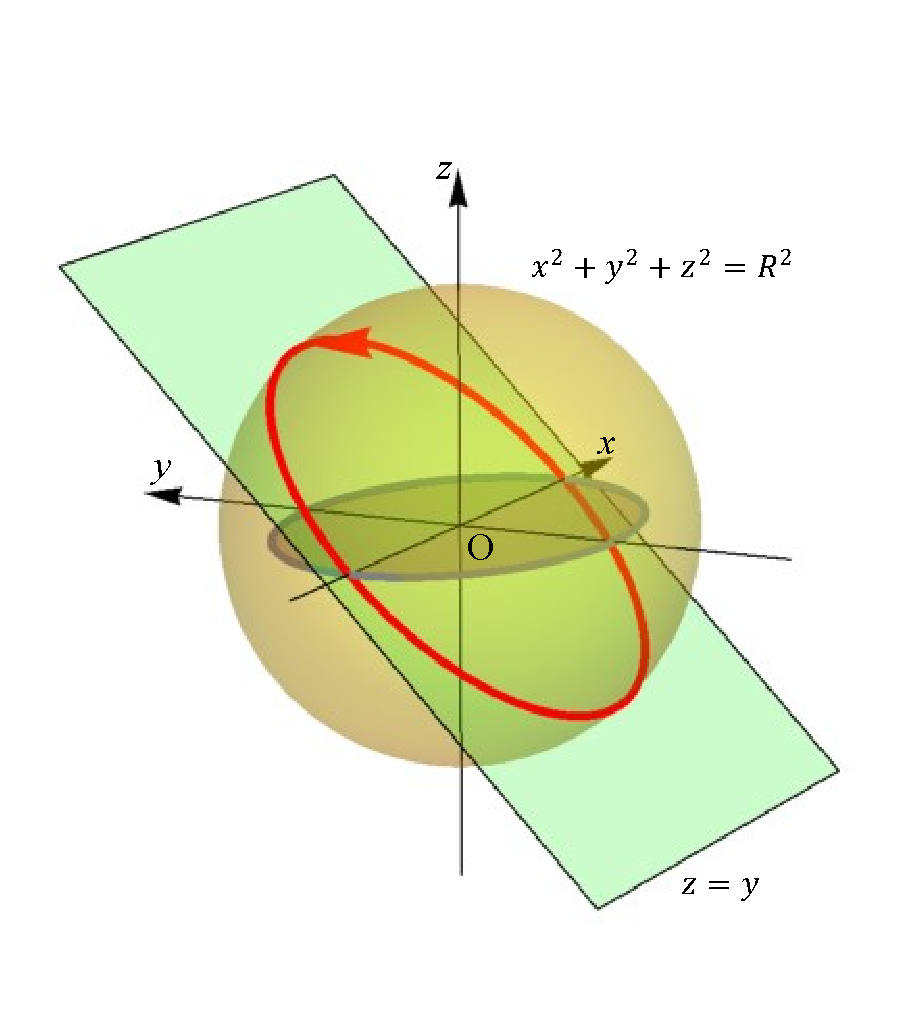
\includegraphics[height=0.7\textheight]{Figures22/Fig13-2-7.pdf}
\end{center}
\caption{习题13.2 7.题图示}
\label{13-2-7}
\end{figure}

解:由$\begin{cases}
x^2+y^2+z^2=1,\\
z=y,
\end{cases}$得$L$所在的投影柱面为$x^2+2y^2=1$,故$L$的方程可表示为$\begin{cases}
x^2+2y^2=1,\\
z=y,
\end{cases}$故可令$L:\begin{cases}
x=\cos\theta,\\
y=\frac1{\sqrt2}\sin\theta,\\
z=\frac1{\sqrt2}\sin\theta,
\end{cases}\theta:0\rightarrow2\pi$,

$\therefore\BLOInt L{xyz\mathrm dz}=\Int0{2\pi}{\cos\theta\frac1{\sqrt2}\sin\theta\cdot\frac1{\sqrt2}\sin\theta}{\frac1{\sqrt2}\sin\theta}=\Int0{2\pi}{\cos\theta\frac1{\sqrt2}\sin\theta\cdot\frac1{\sqrt2}\sin\theta\cdot\frac1{\sqrt2}\cos\theta}\theta\\
=\frac1{2\sqrt2}\Int0{2\pi}{\sin^2\theta\cos^2\theta}\theta=\frac1{2\sqrt2}\cdot4\Int0{\frac\pi2}{\sin^2\theta\cos^2\theta}\theta=\frac1{2\sqrt2}\Int0{\frac\pi2}{\sin^22\theta}\theta\\
=\frac1{2\sqrt2}\cdot\frac12\Int0{\frac\pi2}{\sin^22\theta}{(2\theta)}=\frac1{2\sqrt2}\cdot\frac12\Int0\pi{\sin^2\varphi}{\varphi}=\frac1{2\sqrt2}\Int0{\frac\pi2}{\sin^2\varphi}{\varphi}=\frac1{2\sqrt2}\cdot\frac12\cdot\frac\pi2=\frac\pi{8\sqrt2}$.

\item计算$\BLInt L{\frac{\mathrm dx+\mathrm dy}{|x|+|y|}}$,其中$L$为$|x|+|y|=1$,逆时针方向为正.

\begin{figure}[H]
\begin{center}
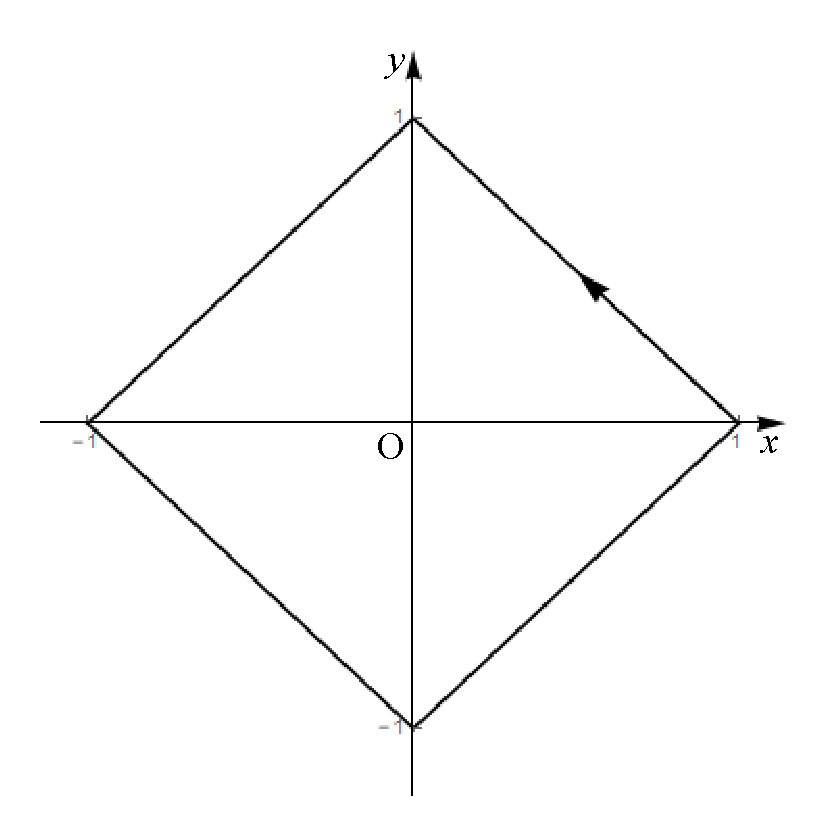
\includegraphics[height=0.3\textheight]{Figures22/Fig13-2-8.pdf}
\end{center}
\caption{习题13.2 8.题图示}
\label{13-2-8}
\end{figure}

解:方法1:$L$的方程$|x|+|y|=1$等价于$y=\begin{cases}
1-x,&0\leqslant x<1,\\
1+x,&-1\leqslant x<0,\\
-1-x,&-1<x\leqslant0,\\
x-1,&0<x\leqslant1,
\end{cases}$

$\therefore\BLInt L{\frac{\mathrm dx+\mathrm dy}{|x|+|y|}}=\BLInt L{\mathrm dx+\mathrm dy}\\
=\varBLInt01{\mathrm dx+\mathrm d(1-x)}+\varBLInt0{-1}{\mathrm dx+\mathrm d(1+x)}+\varBLInt{-1}0{\mathrm dx+\mathrm d(-1-x)}+\varBLInt01{\mathrm dx+\mathrm d(x-1)}\\
=\varBLInt01{\mathrm dx-\mathrm dx}+\varBLInt0{-1}{\mathrm dx+\mathrm dx}+\varBLInt{-1}0{\mathrm dx-\mathrm dx}+\varBLInt01{\mathrm dx+\mathrm dx}\\
=0+2\varBLInt0{-1}{\mathrm dx}+0+2\varBLInt01{\mathrm dx}=-2+2=0$.

方法2:$\BLInt L{\frac{\mathrm dx+\mathrm dy}{|x|+|y|}}=\BLInt L{\frac{\mathrm dx+\mathrm dy}1}=\BLInt L{\mathrm dx+\mathrm dy}=\varIInt D{(\ppx1+\ppy1)}xy=0$, 

其中$D$是$L$围成的区域.

方法3:$\because\md(x+y)=\md x+\md y$,

$\therefore\BLOInt L{\frac{\mathrm dx+\mathrm dy}{|x|+|y|}}=\BLOInt L{\frac{\mathrm dx+\mathrm dy}1}=\BLOInt L{\mathrm dx+\mathrm dy}=0$.

\item计算$\BLOInt L{(y^2-z^2)\md x+(z^2-x^2)\md y+(x^2-y^2)\md z}$,其中$L$为$x^2+y^2+z^2=1$在第一卦限与三个坐标面的交线,方向是$A(1,0,0)\rightarrow B(0,1,0)\rightarrow C(0,0,1)\rightarrow A(1,0,0)$.

\begin{figure}[H]
\begin{center}
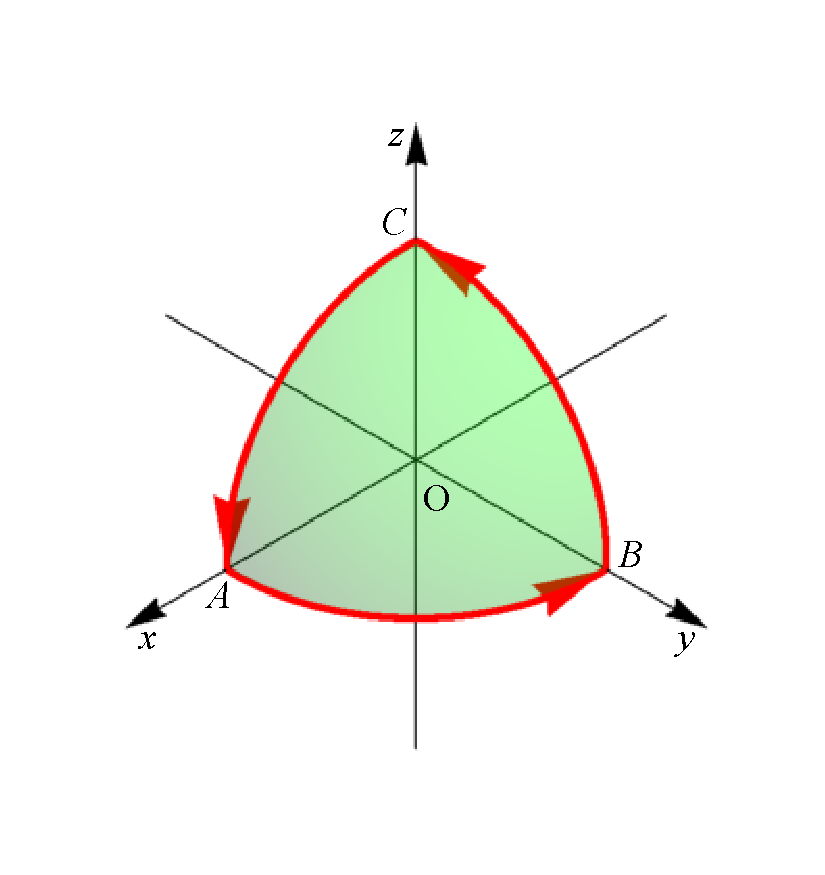
\includegraphics[height=0.7\textheight]{Figures22/Fig13-2-9.pdf}
\end{center}
\caption{习题13.2 9.题图示}
\label{13-2-9}
\end{figure}

解:$\BLOInt L{(y^2-z^2)\md x+(z^2-x^2)\md y+(x^2-y^2)\md z}\\
=(\varint\nolimits_{\overset{\frown}{AB}}+\varint\nolimits_{\overset{\frown}{BC}}+\varint\nolimits_{\overset{\frown}{CA}})[(y^2-z^2)\md x+(z^2-x^2)\md y+(x^2-y^2)\md z]\\
=\BLInt{\overset{\frown}{AB}}{(y^2-0^2)\md x+(0^2-x^2)\md y+(x^2-y^2)\md 0}\\
+\BLInt{\overset{\frown}{BC}}{(y^2-z^2)\md 0+(z^2-0^2)\md y+(0^2+y^2)\md z}\\
+\BLInt{\overset{\frown}{CA}}{(0^2-z^2)\md x+(z^2-x^2)\md 0+(x^2-0^2)\md z}\\
=\BLInt{\overset{\frown}{AB}}{y^2\md x-x^2\md y}+\BLInt{\overset{\frown}{BC}}{z^2\md y-y^2\md z}+\BLInt{\overset{\frown}{CA}}{x^2\md z-z^2\md x}\\
\Big(=\varint\limits_{\substack{x^2+y^2=1,z=0\\ x\geqslant0,y\geqslant0}}{y^2\md x-x^2\md y}+\varint\limits_{\substack{y^2+z^2=1,x=0\\ y\geqslant0,z\geqslant0}}{z^2\md y-y^2\md z}+\varint\limits_{\substack{z^2+x^2=1,y=0\\ z\geqslant0,x\geqslant0}}{x^2\md z-z^2\md x}\\
=\footnotemark\footnotetext{这里的依据是轮换对称性,即按照$x\rightarrow y,y\rightarrow z,z\rightarrow x$可将等号左边第一项变换成第二项,因表达式的值与数学符号无关,故第一项和第二项相等. 同理,按照$x\rightarrow y,y\rightarrow z,z\rightarrow x$可将等号左边第三项变成第一项,故第三项和第一项相等. 变换顺序可用图~\ref{13-2-9-footnote}表示.

\begin{figure}[H]
\begin{center}
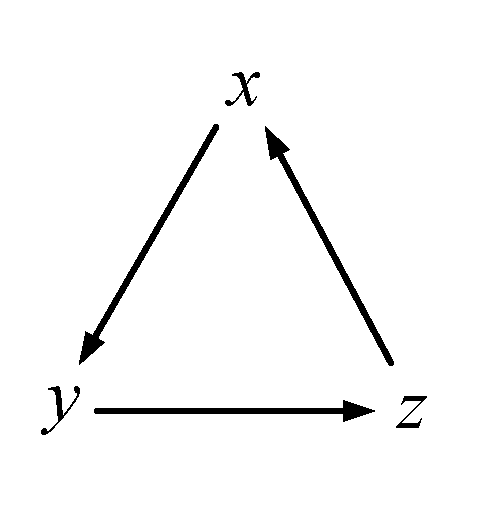
\includegraphics[height=0.2\textheight]{Figures22/Fig13-2-9-footnote.pdf}
\end{center}
\caption{轮换对称性的变换顺序}
\label{13-2-9-footnote}
\end{figure}

}3\varint\limits_{\substack{x^2+y^2=1,z=0\\ x\geqslant0,y\geqslant0}}{y^2\md x-x^2\md y}\Big)\\
=3\BLInt{\overset{\frown}{AB}}{y^2\md x-x^2\md y}\\
=3\varBLInt0{\frac\pi2}{\sin^2\theta\md\cos\theta-\cos^2\theta\md\sin\theta}=3\varBLInt0{\frac\pi2}{-\sin^2\theta\sin\theta\md\theta-\cos^2\theta\cos\theta\md\theta}\\
=-3\Int0{\frac\pi2}{\sin^3\theta}\theta-3\Int0{\frac\pi2}{\cos^3\theta}\theta=-3\cdot\frac23-3\cdot\frac23=-4$.

\item设平面上的力场$\bm F(x,y)$指向原点,每点处力的大小与该点到原点的距离成正比,比例系数为$k$. 设一单位质量的质点沿曲线$\frac{x^2}{a^2}+\frac{y^2}{b^2}=1$从点$A(a,0)$到$B(0,b)$,求力场$\bm F(x,y)$所做的功.

解:因$\bm F(x,y)$指向原点,故可设$\bm F(x,y)=-\lambda(x,y),\lambda>0$,

$\because$每点处力的大小$|\bm F(x,y)|$与该点到原点的距离成正比,比例系数为$k$,

$\therefore|\bm F(x,y)|=\lambda\sqrt{x^2+y^2}=k\sqrt{x^2+y^2}$,

$\therefore\lambda=k,\bm F(x,y)=-k(x,y)=(-kx,-ky)$,

$\therefore$力场$\bm F(x,y)$所做的功
\[\begin{split}
W&=\textcolor{red}{\LLInt{L(A)}{B}{\bm F(x,y)\bm\cdot}{\bm l}=\varBLInt{L(A)}{B}{(-kx,-ky)\bm\cdot(\mathrm dx,\mathrm dy)}=\varBLInt{L(A)}{B}{-kx\mathrm dx-ky\mathrm dy}}\\
&=\varBLInt0{\frac\pi2}{-ka\cos\theta\mathrm d(a\cos\theta)-kb\sin\theta\mathrm d(b\sin\theta)}\\
&=\varBLInt0{\frac\pi2}{-ka\cos\theta(-a\sin\theta)\mathrm d\theta-kb\sin\theta(b\cos\theta)\mathrm d\theta}\\
&=\Int0{\frac\pi2}{(ka^2\sin\theta\cos\theta-kb^2\sin\theta\cos\theta)}\theta\\
&=k(a^2-b^2)\Int0{\frac\pi2}{\sin\theta\cos\theta}\theta=k(a^2-b^2)\Int0{\frac\pi2}{\sin\theta}{\sin\theta}\\
&=k(a^2-b^2)\frac12\sin^2\theta\big|_0^{\frac\pi2}=\frac12k(a^2-b^2).
\end{split}\]
\item计算$\BLInt L{y\mathrm dx+z\mathrm dy+x\mathrm dx}$,其中$L$是螺旋线$x=a\cos t,y=a\sin t,z=bt(0\leqslant t\leqslant2\pi)$,正向为$t$增加的方向.

解:$\BLInt L{y\mathrm dx+z\mathrm dy+x\mathrm dz}=\varBLInt0{2\pi}{a\sin t\mathrm d(a\cos t)+bt\mathrm d(a\sin t)+a\cos t\mathrm d(bt)}\\
=\varBLInt0{2\pi}{a\sin t(-a\sin t)\mathrm dt+bta\cos t\mathrm dt+ab\cos t\mathrm dt}\\
=-a^2\Int0{2\pi}{\sin^2t}t+ab\Int0{2\pi}{t\cos t}t+ab\Int0{2\pi}{\cos t}t\\
=-4a^2\Int0{\frac\pi2}{\sin^2t}t+ab\Int0{2\pi}{t}{\sin t}+0\\
=-4a^2\cdot\frac12\cdot\frac\pi2+ab(t\sin t\big|_0^{2\pi}-\Int0{2\pi}{\sin t}t)=-\pi a^2+(0-0)=-\pi a^2$.
\end{enumerate}
\subsection{习题13.3解答}
\begin{enumerate}
\item用格林公式计算下列积分:\\
(1)$\BLOInt L{xy^2\md y-x^2y\md x}$,其中$L$为圆周$x^2+y^2=a^2$,逆时针方向;\\
(2)$\BLOInt L{(3x+y)\md y-(x-y)\md x}$,其中$L$为圆周$(x-1)^2+(y-4)^2=9$;\\
(3)$\BLOInt L{(x^2+y^2)\md x+(y^2-x^2)\md y}$,其中$L$是区域$D$的边界正向(逆时针),区域$D$由直线$y=0,x=1,y=x$围成;\\
(4)$\BLOInt L{(2xy-x^2)\md x+(x+y^2)\md y}$,其中$L$是区域$D$的边界正向,区域$D$由曲线$x=y^2,y=x^2$围成;\\
(5)$\BLOInt L{(x+y)\md x+xy\md y}$,其中$L$为椭圆周$\frac{x^2}{a^2}+\frac{y^2}{b^2}=1$,正向;\\
(6)$\BLOInt L{\sqrt{x^2+y^2}\md x+[x+y\ln(x+\sqrt{x^2+y^2})]\md y}$,其中$L$为圆周$(x-2)^2+y^2=1$,逆时针方向;\\
(7)$\BLOInt L{\mathrm e^x[(1-\cos y)\md x-(y-\sin y)\md y]}$,其中$L$为$D=\Set{(x,y)}{0\leqslant x\leqslant\pi,0\leqslant y\leqslant\sin x}$的正向边界.

解:(1)设$D$为以$L$为边界的有界闭域,

$\because\frac{\partial(xy^2)}{\partial x}=y^2,\ \frac{\partial(-x^2y)}{\partial y}=-x^2$均在$D$上连续,

$\therefore\BLOInt L{xy^2\md y-x^2y\md x}=\varIInt D{[\frac{\partial(xy^2)}{\partial x}-\frac{\partial(-x^2y)}{\partial y}]}xy=\varIInt D{(y^2+x^2)}xy=\Int0{2\pi}{}\theta\Int0a{r^2\cdot r}r\\
=2\pi\cdot\frac14r^4\big|_0^a=\frac\pi2a^4$.

(2)设$D$为以$L$为边界的有界闭域,

$\because\frac{\partial(3x+y)}{\partial x}=3,\ \frac{\partial[-(x-y)]}{\partial y}=1$均在$D$上连续,

$\therefore\BLOInt L{(3x+y)\md y-(x-y)\md x}=\IInt D{\{\frac{\partial(3x+y)}{\partial x}-\frac{\partial[-(x-y)]}{\partial y}\}}xy=\IInt D{(3-1)}xy=2\IInt D{}xy\\
=2\pi\cdot9=18\pi$.

(3)$\because\frac{\partial(y^2-x^2)}{\partial x}=-2x,\ \frac{\partial(x^2+y^2)}{\partial y}=2y$均在$D$上连续,

$\therefore\BLOInt L{(x^2+y^2)\md x+(y^2-x^2)\md y}=\varIInt D{[\frac{\partial(y^2-x^2)}{\partial x}-\frac{\partial(x^2+y^2)}{\partial y}]}xy=\varIInt D{(-2x-2y)}xy\\
=\Int01{}x\Int0x{(-2x-2y)}y=\Int01{(-2xy-y^2)\big|_0^x}x=\Int01{-2x^2-x^2}x=-3x^3\big|_0^1=-3$.

\begin{figure}[H]
\begin{center}
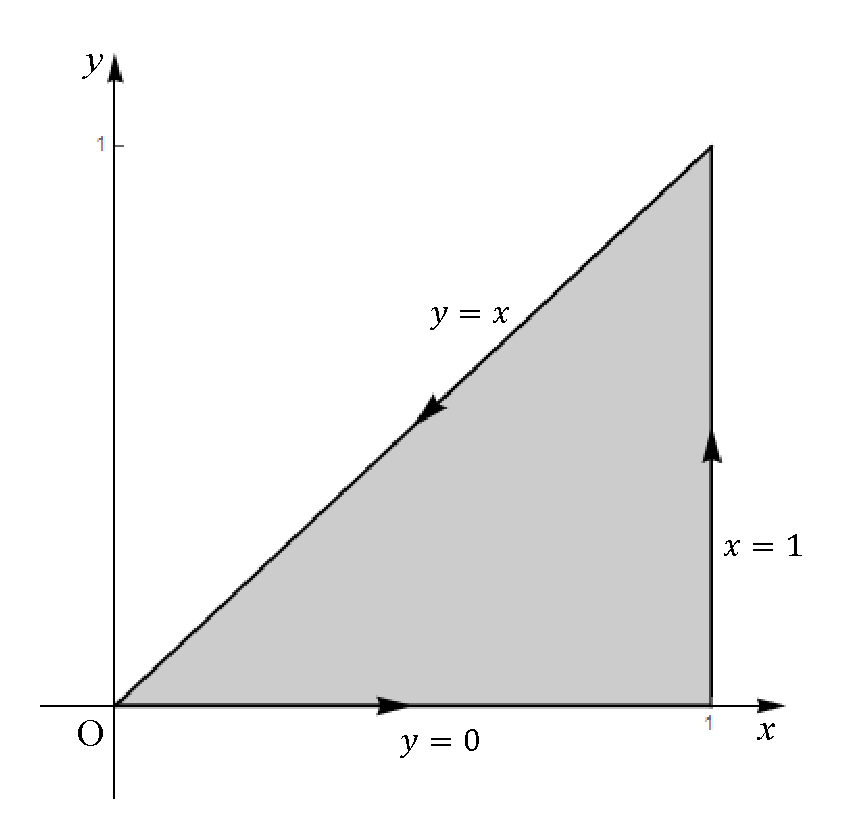
\includegraphics[height=0.3\textheight]{Figures22/Fig13-3-1-3.pdf}
\end{center}
\caption{习题13.3 1.(3)题图示}
\label{13-3-1-3}
\end{figure}

(4)$\because\frac{\partial(x+y^2)}{\partial x}=1,\ \frac{\partial(2xy-x^2)}{\partial y}=2x$均在$D$上连续,

$\therefore\BLOInt L{(2xy-x^2)\md x+(x+y^2)\md y}=\varIInt D{[\frac{\partial(x+y^2)}{\partial x}-\frac{\partial(2xy-x^2)}{\partial y}]}xy=\varIInt D{(1-2x)}xy\\
=\Int01{}x\Int{x^2}{\sqrt x}{(1-2x)}y=\Int01{(y-2xy)\big|_{x^2}^{\sqrt x}}x=\Int01{(\sqrt x-x^2-2x^{\frac32}+2x^3)}x\\
=(\frac1{1+\frac12}x^{1+\frac12}-\frac13x^3-\frac2{1+\frac32}x^{\frac32+1}+\frac24x^4)\big|_0^1=\frac23-\frac13-\frac45+\frac12=\frac1{30}$.

\begin{figure}[H]
\begin{center}
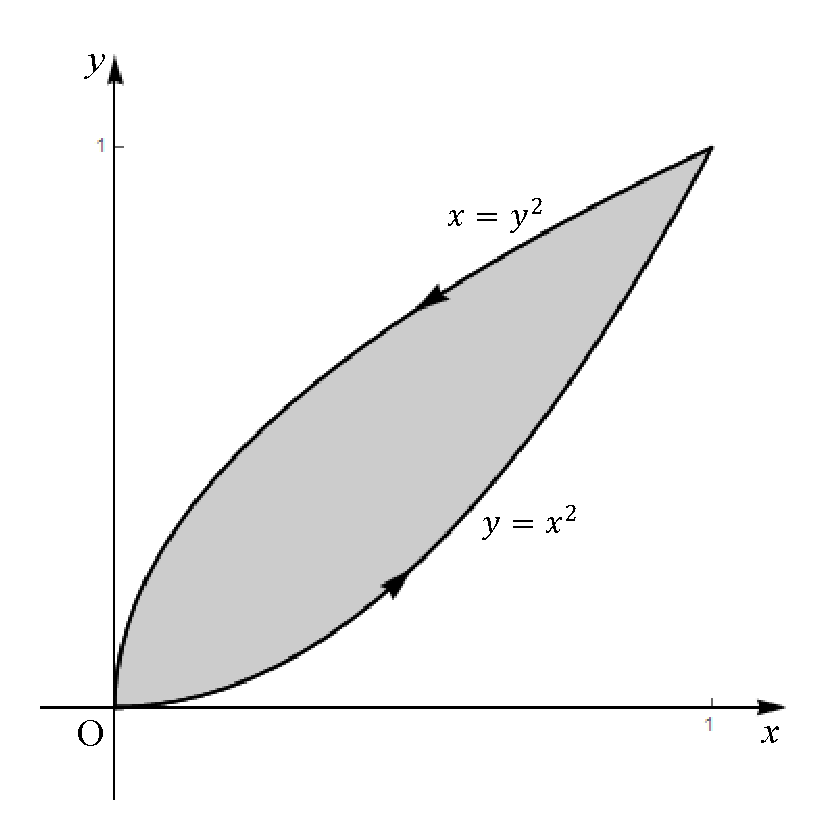
\includegraphics[height=0.3\textheight]{Figures22/Fig13-3-1-4.pdf}
\end{center}
\caption{习题13.3 1.(4)题图示}
\label{13-3-1-4}
\end{figure}

(5)设$D$为以$L$为边界的有界闭域,

$\because\frac{\partial(xy)}{\partial x}=y,\ \frac{\partial(x+y)}{\partial y}=1$均在$D$上连续,

$\therefore\BLOInt L{(x+y)\md x+xy\md y}=\varIInt D{[\frac{\partial(xy)}{\partial x}-\frac{\partial(x+y)}{\partial y}]}xy=\varIInt D{(y-1)}xy\\
=\Int0{2\pi}{}\theta\Int01{(br\sin\theta-1)\cdot abr}r=ab^2\Int0{2\pi}{\sin\theta}\theta\Int01{r^2}r-ab\Int0{2\pi}{}\theta\Int01rr\\
=0-ab2\pi\cdot\frac12=-\pi ab$.

(6)设$D$为以$L$为边界的有界闭域,

$\because\frac{\partial[x+y\ln(x+\sqrt{x^2+y^2})]}{\partial x}=1+y\frac{1+\frac x{\sqrt{x^2+y^2}}}{x+\sqrt{x^2+y^2}}=1+y\frac{\frac{\sqrt{x^2+y^2}+x}{\sqrt{x^2+y^2}}}{x+\sqrt{x^2+y^2}}=1+\frac y{\sqrt{x^2+y^2}},\ \frac{\partial\sqrt{x^2+y^2}}{\partial y}=\frac y{\sqrt{x^2+y^2}}$均在$D$上连续,

$\therefore\BLOInt L{\sqrt{x^2+y^2}\md x+[x+y\ln(x+\sqrt{x^2+y^2})]\md y}=\varIInt D{\{\frac{\partial[x+y\ln(x+\sqrt{x^2+y^2})]}{\partial x}-\frac{\partial\sqrt{x^2+y^2}}{\partial y}\}}xy\\
=\varIInt D{(1+\frac y{\sqrt{x^2+y^2}}-\frac y{\sqrt{x^2+y^2}})}xy
=\varIInt D{}xy=\pi$.

(7)$\because\frac{\partial[-\mathrm e^x(y-\sin y)]}{\partial x}=-\mathrm e^x(y-\sin y),\ \frac{\partial[\mathrm e^x(1-\cos y)]}{\partial y}=\mathrm e^x\sin y$均在$D$上连续,

$\therefore\BLOInt L{\mathrm e^x[(1-\cos y)\md x-(y-\sin y)\md y]}=\varIInt D{\{\frac{\partial[-\mathrm e^x(y-\sin y)]}{\partial x}-\frac{\partial[\mathrm e^x(1-\cos y)]}{\partial y}\}}xy\\
=\varIInt D{[-\mathrm e^x(y-\sin y)-\mathrm e^x\sin y]}xy=\varIInt D{-\mathrm e^xy}xy=-\Int0\pi{}x\Int0{\sin x}{\mathrm e^xy}y=-\Int0\pi{\mathrm e^x\frac12y^2\big|_0^{\sin x}}x\\
=-\frac12\Int0\pi{\mathrm e^x\sin^2x}x=-\frac12\Int0\pi{\sin^2x}{\mathrm e^x}=-\frac12\mathrm e^x\sin^2x\big|_0^\pi+\frac12\Int0\pi{\mathrm e^x}{\sin^2x}=\frac12\Int0\pi{\mathrm e^x2\sin x\cos x}x\\
=\frac12\Int0\pi{\mathrm e^x\sin2x}x=\frac12\Int0\pi{\sin2x}{\mathrm e^x}=\frac12\mathrm e^x\sin2x\big|_0^\pi-\frac12\Int0\pi{\mathrm e^x}{\sin2x}=-\frac12\Int0\pi{\mathrm e^x2\cos2x}x\\
=-\Int0\pi{\cos2x}{\mathrm e^x}=-\mathrm e^x\cos2x\big|_0^\pi+\Int0\pi{\mathrm e^x}{\cos2x}=-\mathrm e^\pi+1-2\Int0\pi{\mathrm e^x\sin2x}x\\
=\frac12\frac1{\frac12+2}(-\mathrm e^\pi+1)=\frac15(1-\mathrm e^\pi)$.

\begin{figure}[H]
\begin{center}
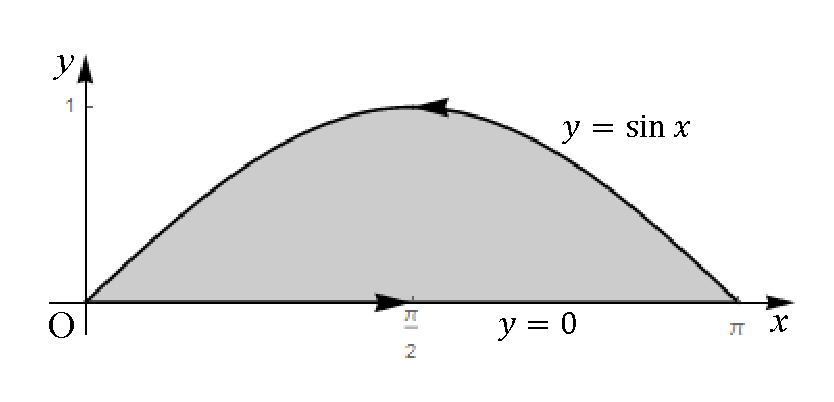
\includegraphics[height=0.2\textheight]{Figures22/Fig13-3-1-7.pdf}
\end{center}
\caption{习题13.3 1.(7)题图示}
\label{13-3-1-7}
\end{figure}

\item计算$I=\BLOInt L{\frac{(x+y)\mathrm dx-(x-y)\mathrm dy}{x^2+y^2}}$,其中$L$:\\
(1)$D=\Set{(x,y)}{r^2\leqslant x^2+y^2\leqslant R^2}(0<r<R)$;\\
(2)$D=\Set{(x,y)}{\frac{x^2}{a^2}+\frac{y^2}{b^2}}$的正向边界.

解:令$Y(x,y)=-\frac{x-y}{x^2+y^2},X(x,y)=\frac{x+y}{x^2+y^2}$,则\[\begin{split}
\frac{\partial Y(x,y)}{\partial x}&=\frac{-(x^2+y^2)+(x-y)\cdot2x}{(x^2+y^2)^2}=\frac{x^2-y^2-2xy}{(x^2+y^2)^2},\\
\frac{\partial X(x,y)}{\partial y}&=\frac{x^2+y^2-(x+y)\cdot2y}{(x^2+y^2)^2}=\frac{x^2-y^2-2xy}{(x^2+y^2)^2}.
\end{split}\]

(1)$\because\frac{\partial Y(x,y)}{\partial x},\frac{\partial X(x,y)}{\partial y}$在$D=\Set{(x,y)}{r^2\leqslant x^2+y^2\leqslant R^2}(0<r<R)$上连续,

$\therefore$
\[I=\varIInt D{[\frac{\partial Y(x,y)}{\partial x}-\frac{\partial X(x,y)}{\partial y}]}xy=0.\]

\begin{figure}[H]
\begin{center}
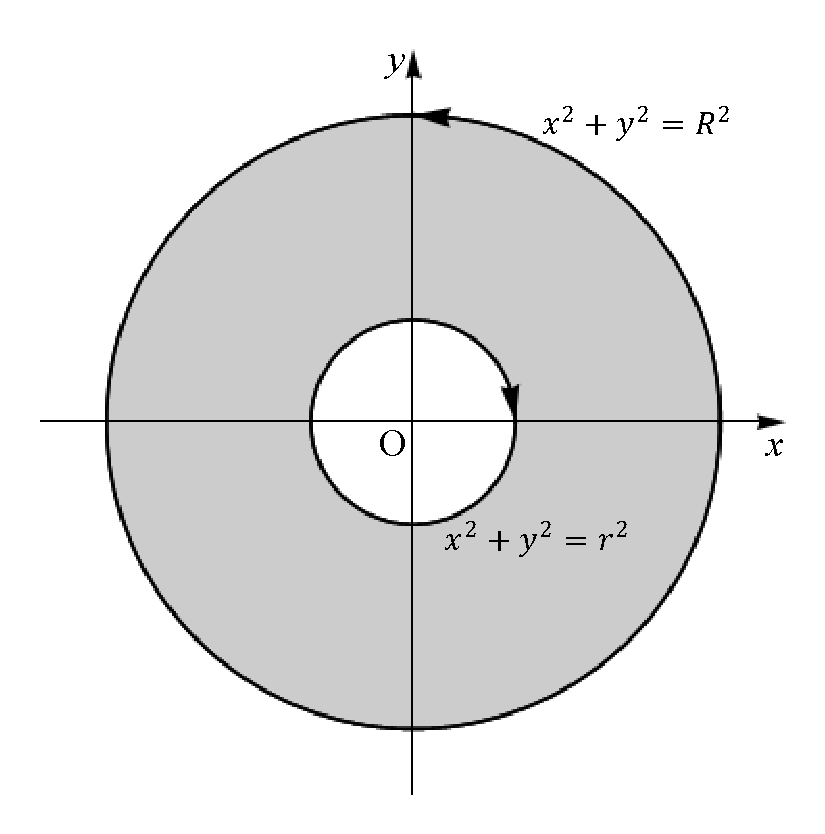
\includegraphics[height=0.3\textheight]{Figures22/Fig13-3-2-1.pdf}
\end{center}
\caption{习题13.3 2.(1)题图示}
\label{13-3-2-1}
\end{figure}

(2)取正向圆周$L_1:x^2+y^2=r^2,r<\min\{a,b\}$,记其围成的区域为$D_1$,则$\frac{\partial Y(x,y)}{\partial x},\frac{\partial X(x,y)}{\partial y}$\\
在$L$和$L_{1-}$围成的区域$D^*$内连续,

$\therefore$
\[\BLOInt{L+L_{1-}}{\frac{(x+y)\mathrm dx-(x-y)\mathrm dy}{x^2+y^2}}=\varIInt{D^*}{[\frac{\partial Y(x,y)}{\partial x}-\frac{\partial X(x,y)}{\partial y}]}xy=0,\]

$\therefore$
\[(\varoint\nolimits_L+\BLOInt{L_{1-}}{)\frac{(x+y)\mathrm dx-(x-y)\mathrm dy}{x^2+y^2}}=I+\BLOInt{L_{1-}}{\frac{(x+y)\mathrm dx-(x-y)\mathrm dy}{x^2+y^2}}=0,\]

$\therefore$
\[\begin{split}
I&=-\BLOInt{L_{1-}}{\frac{(x+y)\mathrm dx-(x-y)\mathrm dy}{x^2+y^2}}=\BLOInt{L_{1+}}{\frac{(x+y)\mathrm dx-(x-y)\mathrm dy}{x^2+y^2}}\\
&=\frac1{r^2}\BLOInt{L_{1+}}{(x+y)\mathrm dx-(x-y)\mathrm dy}\\
&=\frac1{r^2}\varIInt{D_1}{[\frac{\partial(-x+y)}{\partial x}-\frac{\partial(x+y)}{\partial y}]}xy\\
&=\frac1{r^2}\varIInt{D_1}{-2}xy=\frac1{r^2}(-2)\pi r^2=-2\pi.
\end{split}\]

\begin{figure}[H]
\begin{center}
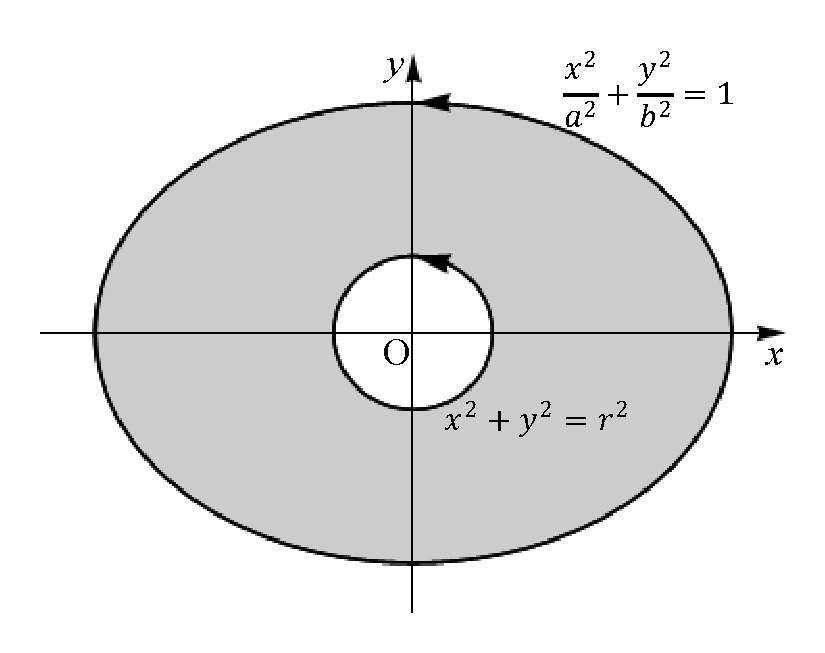
\includegraphics[height=0.3\textheight]{Figures22/Fig13-3-2-2.pdf}
\end{center}
\caption{习题13.3 2.(2)题图示}
\label{13-3-2-2}
\end{figure}
\item设$D$为平面区域,$\partial D$为逐段光滑曲线,$(\bar{x},\bar{y})$是$D$的形心,$D$的面积等于$\sigma(D)$. 试证:\\
(1)$\BLInt{\partial D}{x^2\md y}=2\sigma(D)\bar{x}$;\\
(2)$\BLInt{\partial D}{xy\md y}=\sigma(D)\bar{y}$.

解:(1)$\because x^2,0\in C^1(D)$,

$\therefore\BLInt{\partial D}{x^2\md y}=\BLInt{\partial D}{0\md x+x^2\md y}=\varIInt D{[\frac{\partial(x^2)}{\partial x}-\frac{\partial0}{\partial y}]}xy=\varIInt D{2x}xy=2\varIInt Dxxy=2\sigma(D)\bar{x}$.

(2)$\because xy,0\in C^1(D)$,

$\therefore\BLInt{\partial D}{xy\md y}=\BLInt{\partial D}{0\md x+xy\md y}=\varIInt D{[\frac{\partial(xy)}{\partial x}-\frac{\partial 0}{\partial y}]}xy=\varIInt Dyxy=\sigma(D)\bar{y}$.
\item设$D$为平面区域,$\partial D$为逐段光滑曲线,$f\in C^2(\bar{D})$,求证:
\[
\LOInt{\partial D}{\frac{\partial f}{\partial\bm n}}l=\varIInt D{(\frac{\partial^2f}{\partial x^2}+\frac{\partial^2f}{\partial y^2})}xy.
\]

证明:$\because f\in C^2(\bar{D})$,

$\therefore f\in C^1(\bar{D})$,

$\therefore f$在$\bar{D}$上可微,

$\therefore\frac{\partial f}{\partial\bm n}=\text{grad}f(x,y)\bm\cdot\bm n=(\frac{\partial f(x,y)}{\partial x},\frac{\partial f(x,y)}{\partial y})\bm\cdot\bm n$,

$\therefore$
\[\begin{split}
\LOInt{\partial D}{\frac{\partial f}{\partial\bm n}}l&=\color{red}\LOInt{\partial D}{\text{grad}f(x,y)\bm\cdot\bm n}{l}=\LOInt{\partial D}{(\frac{\partial f(x,y)}{\partial x},\frac{\partial f(x,y)}{\partial y})\bm\cdot\bm n}{l}\\
&=\varIInt{D}{[\frac\partial{\partial x}(\frac{\partial f}{\partial x})+\frac\partial{\partial y}(\frac{\partial f}{\partial y})]}{x}{y}\\
&=\varIInt D{(\frac{\partial^2f}{\partial x^2}+\frac{\partial^2f}{\partial y^2})}xy.
\end{split}\]
\end{enumerate}
\end{document}